\chapter{Technology Review}
\section{OpenAPI}
The OpenAPI specification is a machine readable format for designed to describe RESTful APIs. Being machine readable,
there exists a lot of excellent OpenAPI compliant tooling available to help more efficiently design and test APIs. Our
team made great use of this fact while prototyping our API, generating client stubs, and maintaining
accurate API documentation.

Our API was primarily designed using a web-based tool called Apicurio Studio. Apicurio Studio made it very easy to
visualise the API compared to using traditional text editors. It proved to be an invaluable tool as it allowed the team
to develop the API without having to memorise the entire OpenAPI specification. Apicurio Studio drastically simplified
the process of modifying the various endpoints, their required payloads / responses, HTTP methods, etc. Apicurio Studio
also prompted the team to include documentation whenever creating or modifying components of the OpenAPI file. This
served to enrich the Markdown documentation and client stubs that was also generated from the OpenAPI file.

\begin{figure}[h!]
    \centering
    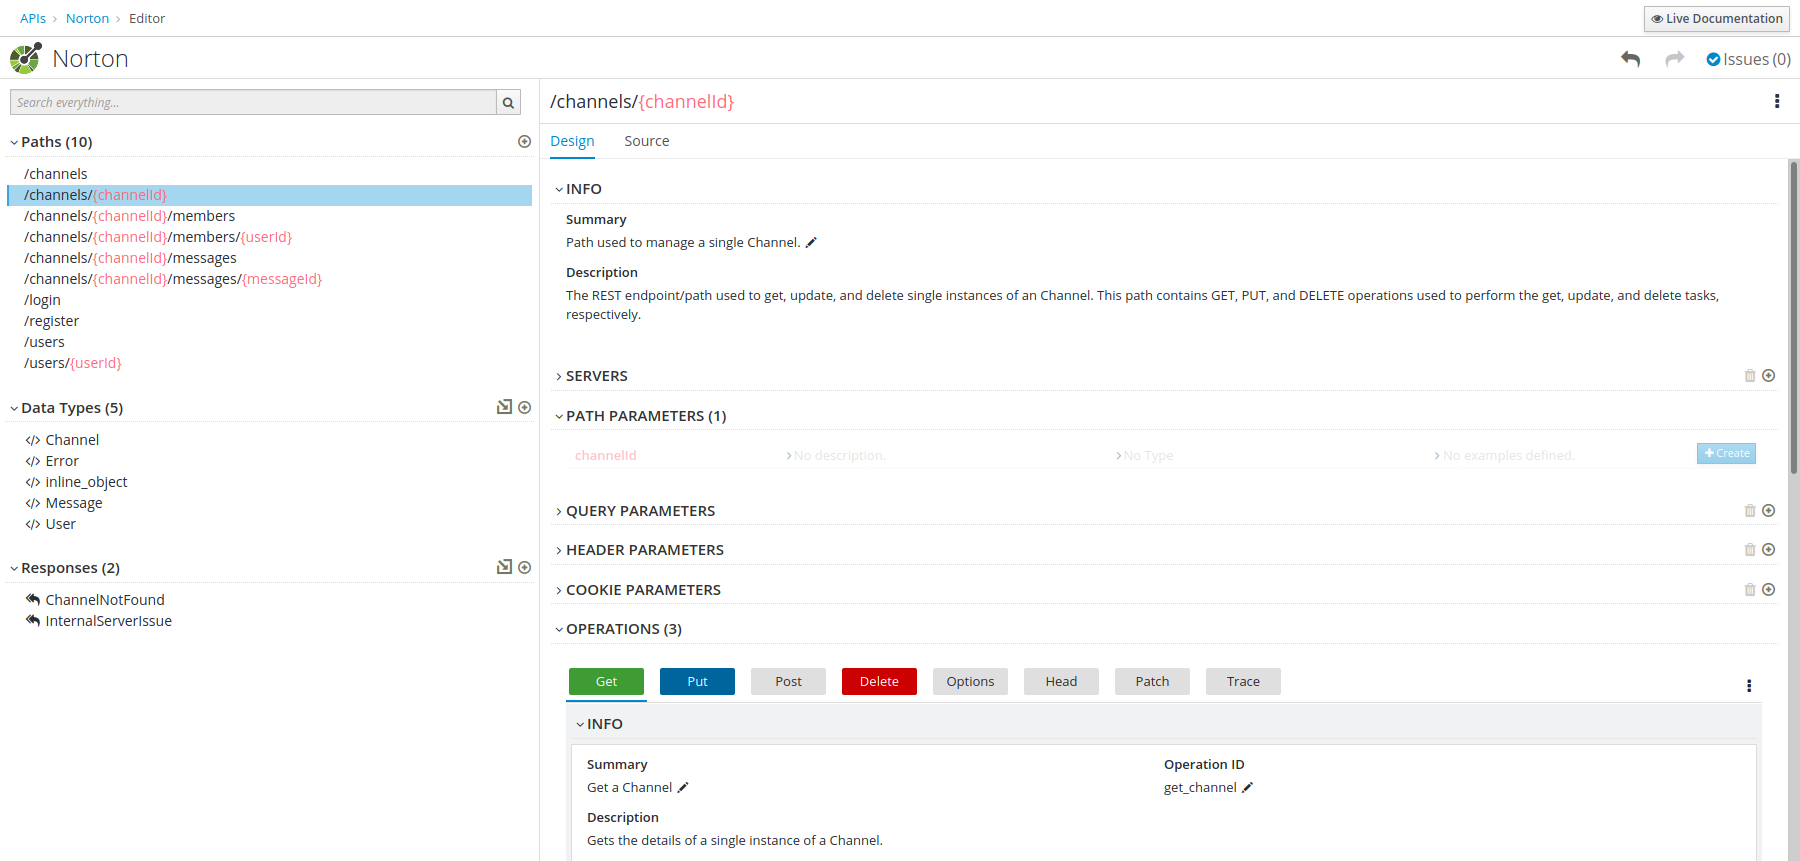
\includegraphics[width=0.7\textwidth]{images/ApicurioStudio.png}
    \caption{Apicurio API Editor}
    \label{image:models}
\end{figure}

\begin{figure}[h!]
    \centering
    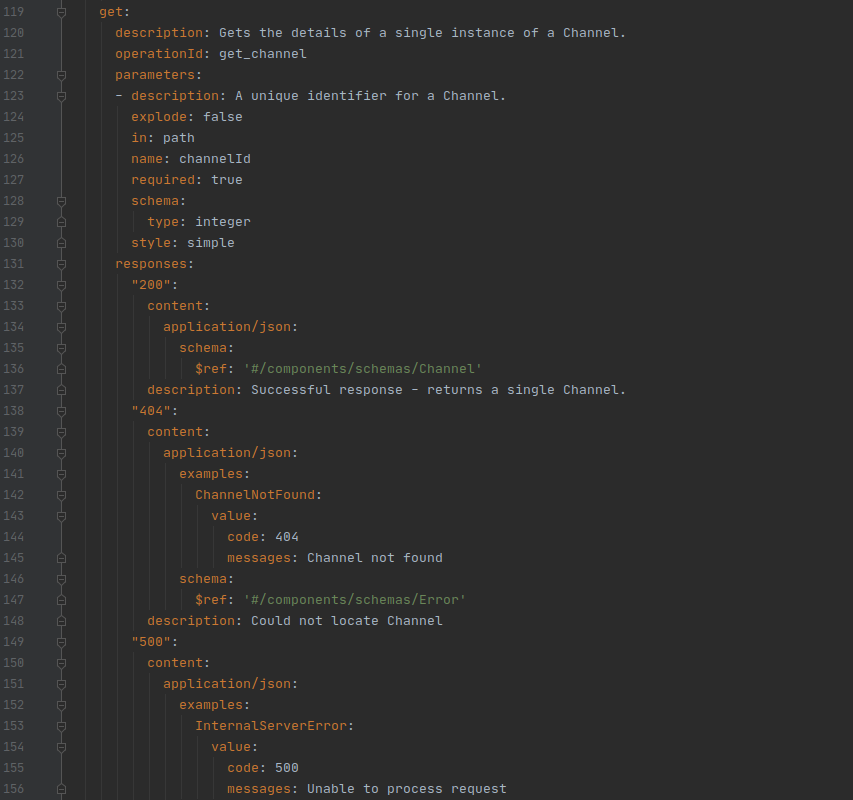
\includegraphics[width=0.7\textwidth]{images/OpenAPI.png}
    \caption{Raw OpenAPI File}
    \label{image:models}
\end{figure}

\section{Version Control Software}

\subsection{Git}
We decided to use git as our version control software of choice. All of our team had experience using git both
personally and for academic use; as such we were satisfied that git would allow use to work collaboratively and
efficiently. By choosing a familiar piece of version control software such as git, it allowed us to focus primarily on
developing the best possible product. Learning to use an entirely new piece of version control software may have been an
interesting endeavour however after briefly considering other options we concluded none of them would not offer any
substantial additional benefits to the project.

\subsection{Github}
Git is inherently a distributed system where every computer in the system has a copy of the entire history of code-base however it is very common practice to also use a centralised git server. Doing so allows each contributor to more easily share their code with others. Contributors can pulling down code-changes from other contributors and pushing their code for others to use. It is possible to create a git server however there are many companies offering hosted git services such as GitHub, Bitbucket, and GitLab. The team opted to use a git server provided by GitHub as it's owned by Microsoft and has developed an excellent reputation for proving secure and reliable services to groups ranging from small teams developing Open Source software to massive multinationals companies who rely on it for their day-to-day operations. As part of GitHub's web interface they also provides auxiliary tooling that is useful for team collaboration such as tools for tracking issues, providing feedback to proposed code changes, distributing releases, etc. GitHub also has very large community of users and a vast amount of documentation, this made GitHub an excellent choice as it was very easy to troubleshoot and find answers to any questions / problems we encountered.

\subsection{Organisations}
To structure of the project it was decided to make use of GitHub's "Organisations" feature. A Github Organisation is
essentially a shared account which is responsible for a series of git repositories on GitHub. GitHub Organisations offer a lot of features which are applicable to groups such as a more robust permissions system. In our case the most attractive feature of a GitHub Organisation was the shared ownership component. Traditionally a project's repository was owned by a single user and any other users may contribute code upstream through pull requests. With the advent of GitHub Organisations the team was better able to share the project as each of the collaborators are all considered owners of the single "VertexChat" organisation and subsequently all of its repositories.

\subsection{Forks}
All of the repositories used in this project belong to the VertexChat organisation. To contribute code each member of
the organisation would first fork the repository they wanted to contribute to and make any code-changes to their own fork. Once a feature was completed they then would submit their code upstream in the form of a pull request. Having individual forks proved to be a very easy workflow to follow and helped keep the project clean and well structured. With each collaborator using their own forks it was possible to avoid a number of issues that can arise when multiple users are committing directly to master. Requiring each member to make pull requests helped ensure overall better code quality.  Pull requests introduced a code review stage for all changes to master by requiring all changes to be approved by another member of the team before it gets merged upstream. GitHub's web-interface makes it very easy to review a pull request and allows comments to be exchanged between reviewers and the contributor as well as clarifications to be made before any code get committed to the master branch.

\section{Flutter}
Flutter is a user interface SDK (Software Development Kit) and also a framework for Dart. Dart is a programming language developed by Google, Flutter is developed by Google.
Both Flutter and Dart are used to build user interfaces that Google are calling widgets. Flutter provides their own pre-configured widgets under catalogs on their website e.g layouts, input and material components. These pre-configured widgets can then be used to build your own widgets to the needs of the application.
With Flutter being an SDK that is set functionalities for the development of an application using it. Development server, hot reload of the app on an emulator or real device and also deployment that will compile the applications code to native code.
Flutter provides DevTools, it is a suite of performance and debugging tools for Dart and Flutter. It can be installed via the CLI or in Android Studio / Intellij, two IDEs made by Intellij.


Flutter was used to develop the user interface for this application. When building the architecture for a mobile application, four main pillars need to be accounted for. These are:
\begin{enumerate}
	\item State Management
	\item Navigation
	\item Inversion Of Control
	\item Data Models
\end{enumerate}

\subsection{State Management}
The goal of state management is to keep the business logic separate from the User Interface (UI), database, network and third-party packages. This is done as the core business logic doesn't change frequently, while the others do.
\\ The UI of an application should not communicate directly with the web. Application Program Interface (API) calls shouldn't be just implemented anywhere. Everything should go through the business logic from a single location.
\\ This is important as it allows a plug-in architecture where you can swap one database framework for another and the rest of the application doesn't even know there was a change. This implementation is useful and important as it makes as it creates a scalable, maintainable and testable app.

\subsection{State Management and Provider}
The architecture for Vertex follows this principle. The business logic in the middle handling the processing of data. The API and the UI with Provider are all completely separate from the business logic and from one another.
\\ The UI, Flutter and Provider are all contained in one part of the app. Flutter itself is a UI framework and Provider is a widget for that framework. Provider is not to be confused with the architecture and is not the state management for the application.
\\ The state is the current values of the apps variables. These are part of the business logic, which is grouped and managed by the model object. From that we can gather that the business logic manages the state, not Provider.

\subsubsection{So, what is Provider?}
Provider is a state management helper. It is a widget that makes some value - such as a state model object, accessible to the widgets below it.
\\ A Consumer widget, which is part of the provider package\cite{provider}, listens for changes in the values and then rebuilds the widgets below itself when changes occur.
See Figure~\ref{image:providerTree}.

\begin{figure}[h!]
    \caption{Tree View of Provider and Consumer Widgets}
    \label{image:providerTree}
    \centering
    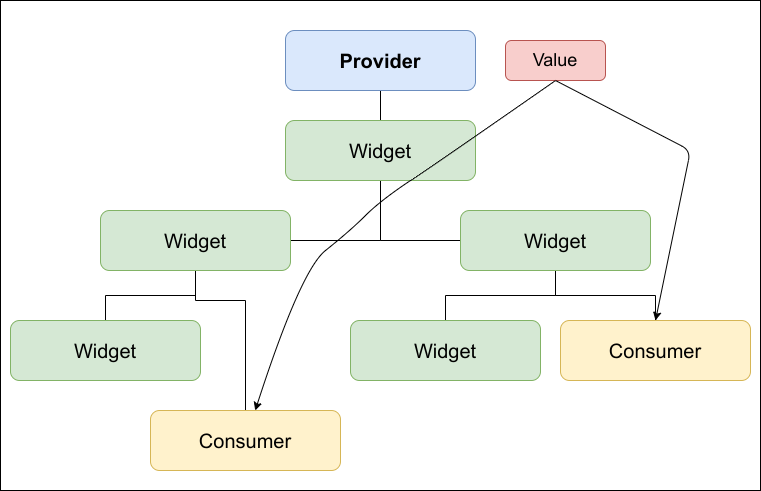
\includegraphics[width=0.9\textwidth]{images/consumer_tree_with_value.png}
\end{figure}

\subsection{Business Logic Communications}
Communication between the UI and business logic is very similar to Model View ViewModel (MVVM) architecture used in most modern day web applications.
\\ The model is the data from a source like a database or WebSocket.
\\ The view is the UI, a Page or widget.
\\ The view model is the business logic which sits in the middle between the UI and the data. Its job is to provide data in a form that the UI can interpret and present, but it knows nothing about the UI itself. This is different from the MVP architecture.
See Figure~\ref{image:mvvmDiagram} and Figure~\ref{image:vertexArch}.

\begin{figure}[h!]
    \caption{Model View ViewModel Diagram}
    \label{image:mvvmDiagram}
    \centering
    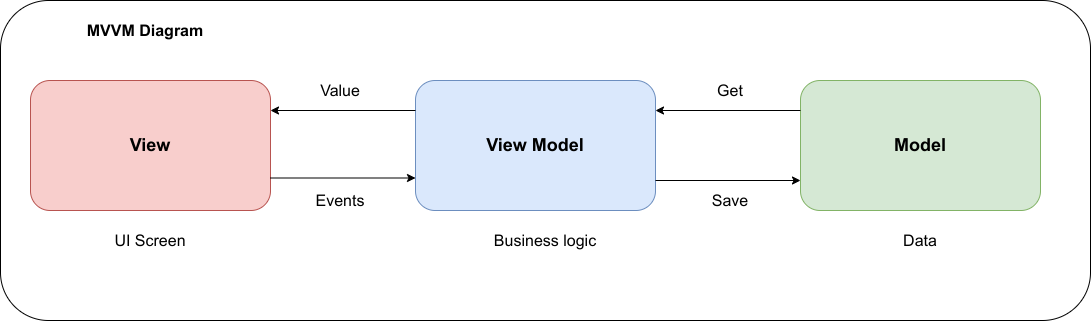
\includegraphics[width=0.9\textwidth]{images/mvvm_diagram.png}
\end{figure}

\subsection{State Management and Bloc}
The Bloc (Business Logic Component) pattern is another state management solution that allows the decoupling of the business logic from the view. Think MVVM(Model-View-ViewModel) pattern but just replace the ViewModel with Bloc. 
See Figure~\ref{image:mvvmDiagram}

\begin{figure}[h!]
    \caption{Bloc Pattern Diagram}
    \label{image:blocPattern}
    \centering
    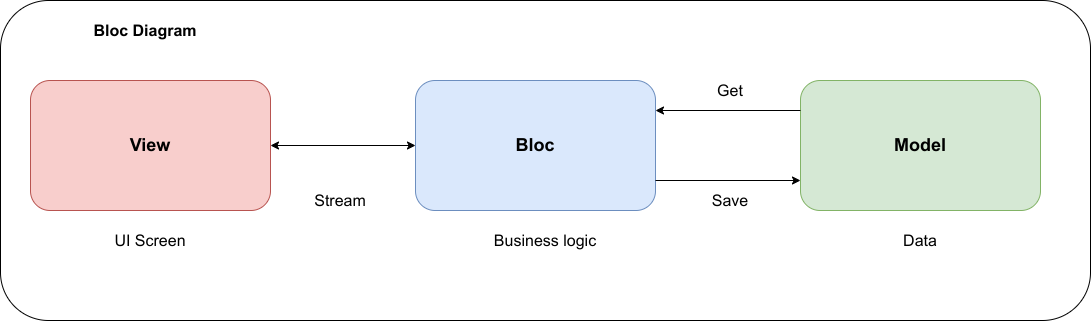
\includegraphics[width=1.0\textwidth]{images/Bloc_diagram.png}
\end{figure}

In Flutter there is no data binding. Instead, the Bloc uses the Streams to expose the data in the view it is needed in. The view waits and listens to the exposed stream and will update its UI accordingly. 

\subsection{Navigation}
Navigation is a key part to any mobile application, however limitations often exist when displaying data in terms of screen real-estate.  Flutter has a few options when it comes to navigation. These are:
\begin{enumerate}
    \item Popping from the stack
    \item Routes
\end{enumerate}

\subsubsection{Popping from the Stack}
As Flutter is built up from a stack of widgets, when you navigate to another page you push a new widget onto the stack, when you go back you'll pop from the stack. 

\subsubsection{Navigation using Routes}
Navigation in Flutter is based around the idea of routes. 
\\ Routes are similar to the routes you would find in a REST API, where each route is relative to some root. In Flutter, the ‘main()’ acts as the route in the application and all other routes are relative to that one. 

\subsection{Inversion Of Control}
Flutter has three main forms of dependency injection to get objects where they are needed. These are:
\begin{enumerate}
    \item Inherited Widget
    \item get\_it
    \item Provider
\end{enumerate}

Dependency injection is writing code that supplies the objects with other objects that they depend on. Typically dependencies are passed through the classes constructor which work fine for accessing data one or two levels down. It becomes an issue when all of a sudden a widget is 5 levels deep in the widget tree and you need access to a data object in a class. 

\subsubsection{Inherited Widget}
Inherited widget is built into Flutter, it is a widget that allows access though the BuildContext to all properties to every widget in its sub-tree. Inherited widget is used in MediaQueries and themes as well as anything else the base app provides.

\subsubsection{get\_it}
'get\_it' is a service locator package developed by the Flutter Community. 'get\_it' is set up by creating a locator.dart file and adding an instance of 'get\_it' globally that can be accessed anywhere it is imported throughout the application. A function the locator class is created which is where services are registered. The function in the locator class is called in the main() function before runApp() is called.
\\ Class types Factory and Singleton can be registered with the service. Factory is where a new instance is returned every time it is called. Singleton keeps a single instance of the resisted service and returns that one each time it is called.

\subsubsection{Provider}
Provider is a Flutter Community based package which is basically an Inherited widget upgrade. It provides types like StreamProvider, ChangeNotifyProvider, ListenableProvider that can be used to build a storage robust architecture for a mobile application.

\subsection{Data Models}
Models are important in any application as the app could work with various types of data. Data models are effective in-memory where screens can fetch data as needed. Dart serialization is also handled in the model class using 'dart:convert' package, '.fromJson()' for constructing a new object from a map structure, and 'toJson()' method which converts an object instance into a map.

\section{WebRTC}
\label{webRTCTR}
Web Real-Time Communication (WebRTC), is an important tool in relation to this project, and offers real-time communication with web-browsers and mobile applications, and is built and managed in an open source fashion. WebRTC offers the likes of direct file sharing, and peer-to-peer media, without the need for an intermediary server or the use of third-party software \cite{johnston2012webrtc}. 
\\The Application Programming Interface (API) developed for WebRTC has the capability to be used in conjunction for development of data, audio, and video channels. The API for WebRTC has three main elements: (i) Peer-Connection, (ii) Data-Channel, (iii) Media-Stream \cite{jesup2015webrtc}. Peer-Connection generates a direct form of communication between users/peers. Data-Channel is the transportation of data as a service between users via a bidirectional peer-to-peer connections. The Media-Stream has the capabilities  to create video and audio streams, and also manages the content of those streams \cite{14003034520191201}.

\section{WebRTC Overview and Terminology}
\subsection{Web Architecture}
The client-server paradigm is generally regarded as the classic semantics for web architecture in which browsers send HTTP requests for content on a web server, with replies with a payload containing the response.
\\The server provides resources which are associated closely with an entity known as a Uniform Resource Identifier (URI), or Uniform Resource Locator (URL).
\\ In the scenario of a web application, JavaScript code can be embedded in HTML to send back to the client, which is interacted with by browsers through a standard JavaScript APIs and through the user interface by end-users \cite{loreto2014real}.

\subsection{WebRTC Architecture}
The schematics for client-server WebRTC are extended between browsers with the introductions of peer-to-peer communication paradigm. The generally used architectural model draws its inspiration from the Session Initiation Protocol Trapezoid. However, the most common scenario for WebRTC is the architectural model depicted in figure~\ref{image:simpleWebRTCSystem} \cite{loreto2014real}.

\subsection{Signaling}
\label{signallingTechR}
Complete specific control of the media plane, while having as much of the signalling plane as possible left to the application layer, is the design idea for WebRTC. The reason being the a variety of applications may opt to use different signaling protocols.
\\ The most important information that needs to be sent is the session description, which specifies the information on transport, as well as the type of media, the format, and the collection of associated media configuration parameters needed to establish paths for media \cite{loreto2014real}.

\subsection{Media Stream}
By definition, a media stream is an actual stream of data which can be audio and/or video, but is represented in an abstract fashion. The purpose of it is to handle actions which manage the media stream, the likes of which include displaying content on the stream, recording content on the stream, or sending content to a remote peer. A media stream can also be extended to represent a remote stream or a local stream. The difference being that one is sent from a local node (remote stream), while the other is sent to a remote node (local stream).
\\ A local media stream is the representation of a media stream sent from a local capture device, i.e. microphone, webcam. Creation and use of a local stream is granted from the web applications request of access from the user through the function getUserMedia(). After which, the application will specify its media type (audio/video) access requirement. Access is either granted or denied based on the devices selector in the browsers interface. Access can be revoked once the application is finished by calling LocalMediaStream’s stop() function.
\\  A break down of the media plane shows that signalling between peers is carried out of band. Secure Real-time Transport Protocol (SRTP) has the function of carrying the media data along with the RTP Control Protocol information which is used in monitoring statistics on transmission associated with streams of data \cite{loreto2014real}.

\subsection{Peer Connection}
Peer Connection allows direct browser to browser communication between peers/users. It is the representation of association with remote peers, which in most cases in an instance of the same application running on the other end. Coordination of communications are through the use of a signaling channel, which is provided by scripting code via the web server. Once a peer connection is established, the remote browser can be sent media streams directly.
\\ Together with the STUN and TURN servers, the ICE protocol let UDP-based media stream traverse NAT boxes and firewalls as a mechanism for Peer Connection. The ICE allows the browsers to discover information about the network topology of where they are deployed to find the best communications path. Upon arrival, the receiving peer connection is fed each signalling message \cite{loreto2014real}.

\subsection{Data Channel}
The Data Channel API provides a transport service for web browsers to allow the exchange of generic data in a bi-direction fashion between peers.
\\ The encapsulation of SCTP over DTLS over UDP along with ICE it provides a system which is NAT traverse-able, and also provides integrity protected transfers and source authentication. This also has the benefit of allowing the parallel media transfers to inter-work smoothly with the data transport.
\\ Each stream is a representation of a logical channel which is unidirectional, and provides an in-sequence delivery. This message sequence can be ordered or un-ordered when sent. The order of the messages is only saved for the ordering of all messages in the same stream.
\\ Setup of the DataChannel is initiated when the function CreateDataChannel() on an instantiated PeerConnection object is called for the first time. Subsequent calls to this function creates new DataChannels within the existing SCTP association \cite{loreto2014real}.

\section{WebRTC Security}
In comparison to some conventional real-time systems, such as SIP-based soft phones, the communications for WebRTC are controlled directly through the use of a Web-Server, which can be interacted through the use of a JavaScript API. See Figure~\ref{image:simpleWebRTCSystem}.
\\Complexity is increased when looking at the likes of inter-domain calling, alongside of which bring a number of security challenges \cite{rescorla2013webrtc}.

\begin{figure}[h!]
    \caption{A Simple WebRTC System.}
    \label{image:simpleWebRTCSystem}
    \centering
    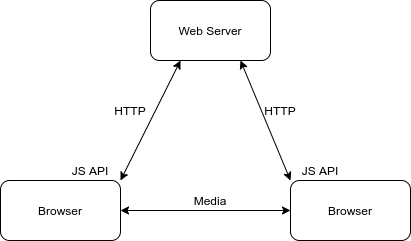
\includegraphics[width=0.5\textwidth]{images/simpleWebRTCSystem.png}
\end{figure}

\subsection{WebRTC Trust Model}
The trust model in WebRTC fundamentally is the hierarchy of trust, which is rooted in the browser, serving as the user’s Trusted Computing Base (TCB). The browser will ultimately enforce any security property the user wishes. On the converse, no security guarantees are possible should the browser be compromised. In an optimal system, reliance on the trust in external entities apart from the browser would not be done, this however, is not possible for a functional WebRTC system. There exist two categories for other networks: The type in which the browser can authenticate, thus granting permissions to resources with otherwise sensitive access, and those which where authentication is infeasible and therefore are un-trusted  \cite{rescorla2013webrtc}.

\subsection{Authenticated Entities}
In the WebRTC system there exists two major categories of authenticated entries:
\begin{itemize}
	\item Calling Services: Sites with a verifiable origin
	\item Other Users: Peers with a cryptography verifiable origin
\end{itemize}
* Note that, however, authentication does not equate to trust. This is in the case of access to device hardware such as webcam or microphone. \cite{rescorla2013webrtc}

\subsection{Unauthenticated Entities}
In cases apart from the entities outlined above, network elements are generally not identifiable, and therefore are un-trust-able. This does not negate the possibility of interaction, instead it means an assumption must be made that interactions are in-feasible \cite{rescorla2013webrtc}.

\subsection{Origin and Web Security Issues}
WebRTC uses the origin as a basic unit of permissions. Due to the security associated with the origin  depending on the ability to authenticate content from the origin, the origin can be securely established only if the data is transferred through HTTPS. Therefore, any client-side must treat HTTP and HTTPS differently in terms of domain permissions \cite{rescorla2013webrtc}.

\subsection{IP Location Privacy}
The default behaviour for ICE has a side effect which leaks large amounts of location information, which is that the peers learns the IP addresses. This ultimately has negative consequences with privacy in most circumstances. Should the user’s IP need to be hidden from the server, a sort of explicit privacy preserving mechanism needs to be implemented on the client, but is unavailable yet for WebRTC \cite{rescorla2013webrtc}.

\subsection{Communications Security}
In a case where the signaling server does not use HTTPS to secure communications, any on-path attacker can substitute its own identity for that of either endpoint by replacing he DTLS-SRTP fingerprints in the handshake.
Even if the application uses HTTPS, a man-in-the-middle attack can be potentially mounted by the signalling server unless a mechanism for independently verifying keys can be implemented \cite{rescorla2013webrtc}.

\section{Use-Cases For WebRTC}
Teleconferencing is an area that encompasses quite a broad spectrum of users. It can range from users simply engaging in a multi-user chat for social reasoning, or can be used in a more professional sense, from the likes of companies engaging with their clients and fellow workers, or to doctors and medical professionals communicating with their clients or fellow specialists. Whatever the use case it is relied on quite heavily on a day to day basis \cite{14003034520191201}.

\subsection{Use-Cases For WebRTC: Medicine}
Teleconferencing, in the field of medicine, for example, allows to reduce the cost of nursing, to overcome shortages for the work force in health care, to maintain a better health care at home, to enhance the health of the public, to generate better education in terms of health, and to create better doctor-patient and inter-professional relationships \cite{14003034520191201}. 
\\Referring back to the field of medicine, WebRTC has been used in the likes of online medical consultation, which aids in the treatment and rehabilitation of patients, and in other cases can be used for diagnosis by transmitting radiology images \cite{14003034520191201}. For the likes of the World Health Organisation, the use of telemedicine can be used to overcome and breakdown geographical barriers in order to increase access to health care services. The initial benefit being in the likes of rural or underdeveloped communities, communities in which would normally lack the access of health care. Through the use of WebRTC based applications, a form of ehealth could be used to transfer health resources and health care through electronic means. However, there are many issues when faced with the implementation of this. The likes of which being due to the inadequacy of the systems being used; the level of service quality to user satisfaction; or possibly even the return on investment in relation to the acquisition cost and system maintenance. \cite{S187705091632345620160101}

\section{WebRTC Communication Protocols}
Figure~\ref{image:webRTCCommsArch}. displays the architecture, at a higher level, used in our application. With this, it is necessary that both parties send the necessary protocol information through a socket in order to create a connection. Interactive Connectivity Establishment (ICE) applicants are proposed and classified through this protocol in order to identify and locate peers. First we need to identify the peer address, this is done with a Session Traversal Utilities for Network Address Translator server. A direct media connection is established only if the STUN server is successful in the identification of addresses. Should that not be the case, a Traversal Using Relays around Network Address Translator server allows in the accessing the peers public address and also in media transferring between peers\cite{14003034520191201}.

\begin{figure}[h!]
    \caption{WebRTC Communications Architecture.}
    \label{image:webRTCCommsArch}
    \centering
    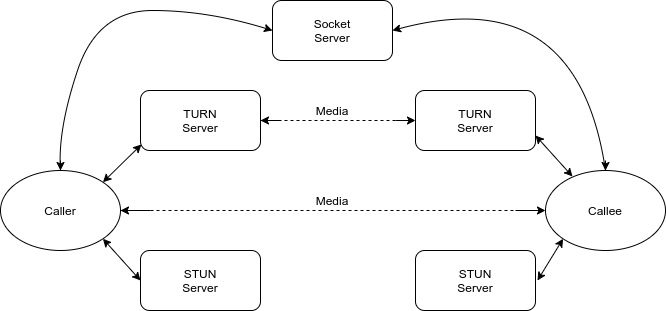
\includegraphics[width=0.9\textwidth]{images/WebRTCCommsArchitecture.png}
\end{figure}

\begin{figure}[h!]
    \caption{Communication Protocol between Peers \cite{14003034520191201}}
    \label{image:commsProtocol}
    \centering
    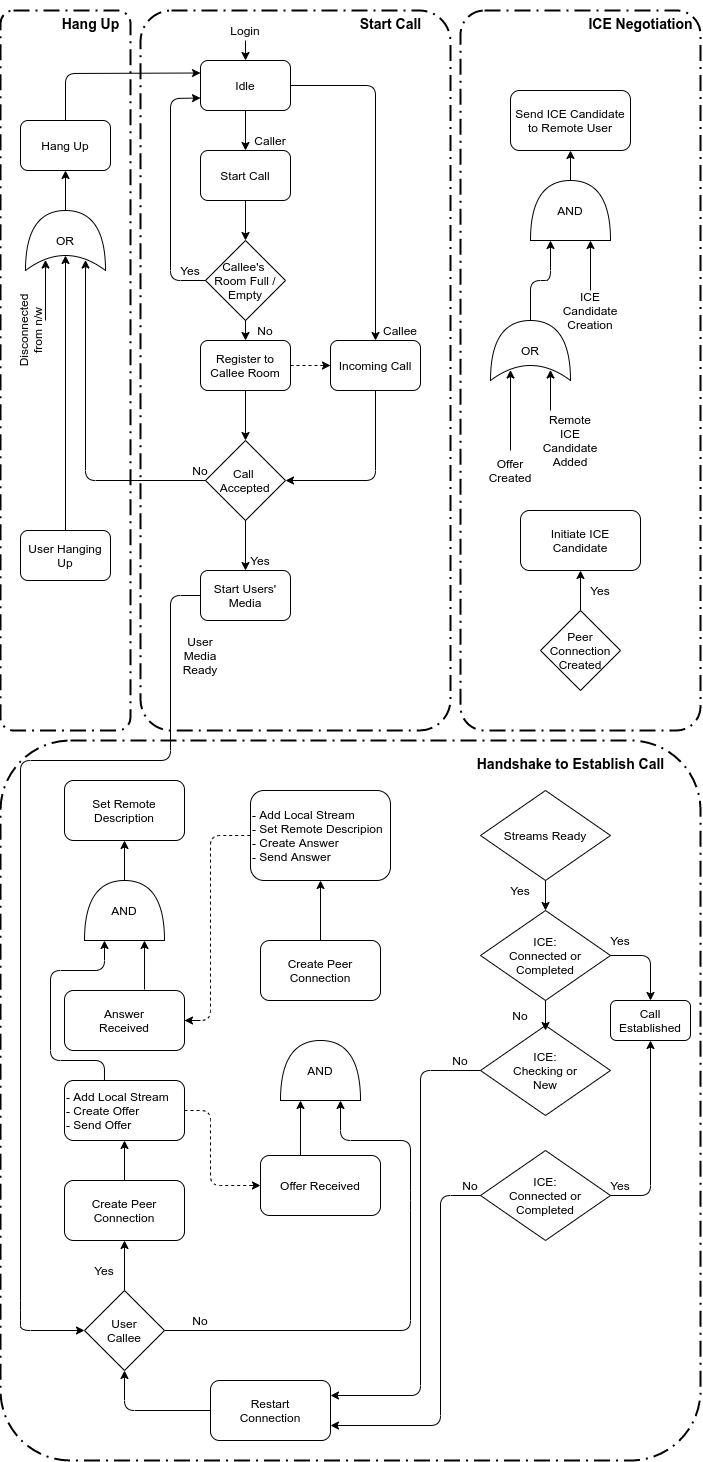
\includegraphics[width=0.8\textwidth]{images/CommunicationProtocol.png}
\end{figure}

Figure~\ref{image:commsProtocol} displays the protocol used in communication to establish a call procedure composed of initiation, handshake, ICE negotiation, and hang-up stages which is used between peers.
In the first stage, initiation, peers are assigned to different rooms by the socket server when they first log in to the application. The purpose of these rooms are to send the status of communication for the users. This is useful because it sets the users up for the Idle step, in which they can receive or initiate calls. The processes of calling starts by registering with the room of the second/third/n peer to which that peer receiving a call. Should it be a case where the callee’s room is either empty or full, the process of calling is terminated. Should this not be the case, the incoming call is received. Only after the call is received is the WebRTC communication procedure started. 
\\The use of the WebRTC library is to send and receive media to or from peers. To begin, the peer initiates their media streams, this can either be audio, video, or both. On completion of this, and on ready of the streams, a peer connection is created by the callee, which is added to its local stream, subsequently creating an offer, and then finally sending this offer to the caller. The same procedure will be followed in the case of the text chat communication by taking the ready state of the peers media stream, without the media starting, and the application should start the data channel of text message transfer. On retrieval of this offer, the caller will create a peer connection. They will set a remote description, add the local stream of the offer, generate and answer and finally will send the answer to the callee. A remote description is set once the answer is received by the callee. ICE candidates are initiated only while a peer connection is set. If a local ICE candidate is generated, the protocol will verify the offer of creation, and will add the ICE candidates remote user. Should one of these checked items be available, the candidates local ICE is sent to the remote user, and subsequently will be added by the remote user as a remote ICE candidate.
\\On ready of local and remote streams, connection states of ICE are controlled. Should the state of ICE be in connected or completed, the call will be generated  and communication screens for audio and video will be presented to the users. If the ICE connection is in a checking or new state, the ICE protocol will wait and check the status periodically. Should this fail i.e the connection is in a different state, then the connection will be closed.
On call close, the connection and channel of data will be closed and all streams will be interrupted. This should terminate the callee’s room, and set the peers in a new state of ready to receive/create a new call \cite{14003034520191201}.

\section{MySQL}
MySQL is an open-source relational database management system. It is a Relational Database Management system (RDBMS). These databases are ACID compliant. They boast recovery and backup, but require an expertise to use. SQL is almost ubiquitous, and is the de-facto standard for data processing. 

\subsection{About Relational Databases}
\label{rdbms}
A relational database is a style of database which stores its data in tables in the format utilising rows and columns. This creates a kind of ease of access. The tables can then relate to one another through the use of keys. The main being a primary key, which is a unique value in the table, commonly denoted through an auto-increment value. Other keys can include a super key, a candidate key, an foreign key and composite/compound keys. 
\\A relational DBMS is generally composed of layers. These layers consist of three tiers. The first being the Physical Layer (Internal), which deals with the bit-level transmission between the different devices, supporting either electrical or mechanical interfaces which are connected to the physical medium for synchronised communication. This layer also handles the file organisation, the indexing, and the clustering. Only one instance of the physical level can exist at any time in an SQL database. On this level the database is organised into records, then into fields. It sits quite close to the systems hardware, copying to main memory when a user queries a record.
\\A relational DBMS is generally composed of layers. These layers consist of three tiers. The first being the Physical Layer (Internal), which deals with the bit-level transmission between the different devices, supporting either electrical or mechanical interfaces which are connected to the physical medium for synchronised communication. This layer also handles the file organisation, the indexing, and the clustering. Only one instance of the physical level can exist at any time in an SQL database. On this level the database is organised into records, then into fields. It sits quite close to the systems hardware, copying to main memory when a user queries a record.
\\The third layer of a relational DBMS is the External Layer (View). This layer consists of the views of the database. It is the highest level in the database. This level incorporates a high level of abstraction, and maintains security of the database by giving users access to only the data they need at a given time.
See Figure~\ref{image:rdbmsLayers}.

\begin{figure}[h!]
    \caption{Layers in a Relational Database.}
    \label{image:rdbmsLayers}
    \centering
    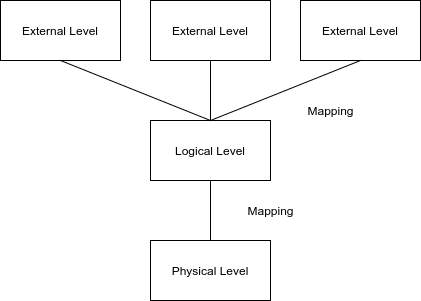
\includegraphics[width=0.8\textwidth]{images/RDBMS_Layers.png}
\end{figure}

\subsection{Why MySQL?}
SQL was chosen for this project because it was felt to be the best fit. Examinations other options such as graph databases, and document stores, took place to confirm this. Examinations of all three and, in the case of this application, only two of the three choices were a fit. The least likely to suit the application was a document store, as it is architecture around storing, retrieving and managing document-oriented information. Since users would be interacting with other users across an array of channels, a relational or graph database was the better choice.  A graph database could have been used and there are many pro’s in the case of our application for using it. For example the relationship of the users, channels, and messages could have been easily represented as a graph, but it was felt that a relational table would do the same job efficiently. Also, since SQL is the standard for data-processing we felt it was the better choice as it is known for its capabilities to handle large amounts of data at any time. This being said, a graph database would have no issues processing the information the application is handling. Ultimately an SQL database was chosen for some of its features such as locking, transactions and the fact that it is ACID compliant.
\\ ACID compliance is used with transactions and is broken down into several parts. The first being Atomicity, which means the transaction is atomic. It either is performed in its entirety, or it isn’t performed at all. The second letter in ACID stands for Consistency, which means that the transaction will transform the database from one consistent state to another. The I stands for Independence, which means that transactions can be executed independently of each other. This is really what was being looked for in terms of a database for this application, as there can be quite a lot of information being exchanged at the same time. This ensures that the correct information is being sent and written securely. The final letter in ACID stands for Durability. This means that only successful transactions are stored permanently to the database. If a transaction is not stored correctly the transaction can be aborted and no formation is stored. This can be a safeguard for when a user experiences a connection loss or any similar situation. See Figure~\ref{image:txLifeCycle}.

\begin{figure}[h!]
    \caption{Life-cycle of a Transaction.}
    \label{image:txLifeCycle}
    \centering
    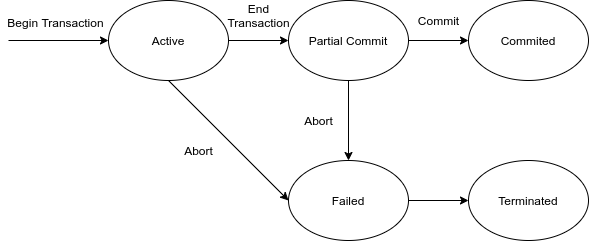
\includegraphics[width=0.8\textwidth]{images/TransactionLifeCycle_ACID.png}
\end{figure}

\section{Firebase \& MySQL - A Comparison}
This section aims to compare Firebase, a real-time database which could have been used for this project as it integrates quite well with Flutter, to the database which was chosen, MySQL. This comparison is based in terms of response time, and performance is compared using CRUD operations for both databases. The operations are analysed from a data standpoint using the Wilcoxon Sinded-Rank test.
\\ MySQL, as outlined above, is a relational database which supports Structured Query Language (SQL). It is regarded as one of the most popular databases used in the world. This is due to it’s open source nature which boasts reliability and compatibility with major hosting providers. It is also quite cost effective, which makes for an ease of management. It has a few drawbacks in terms of scaling, examples of which being development time and logging costs for the database.
\\ In comparison to this, there exists the likes of Firebase, which is a Realtime Database, hosted through the use of Googles Firestore platform. This is a cloud-hosted NoSQL database. The real-time feature of this database provides features such as synchronising across connected devices, and availability of cached data when there is connection issues. This would have been an ideal feature for use in this project, and it was heavily scrutinised in the beginning, but worries arose as feasibility issues arose in terms of WebRTC compatibility. Another advantage to Firebase is the relative ease of use, so apps could be built and deployed without worry of scalability from a design standpoint. The drawback to this is that complex queries and migrations are quite difficult to achieve, where as with MySQL these are achievable with some experience.
\\ Based on several reports of comparisons of other database times: Truica et al(2015)\cite{truica2015performance}; Tang and Fan(2016)\cite{tang2016performance}; and Pereira et al(2017)\cite{pereira2018nosql}; have shown that the execution time for CRUD operations is that MongoDB is the fastest when fetching data. CouchDB is quite good when it comes to intensive write operation. Couchbase has quite powerful data processing. Redis has the top performance for insert and execute operations in comparison to other databases, but has limitations with very large data-sets. In terms of threaded searches, it was shown that Couchbase has a better performance at most operations, except for when retrieving / inserting multiple documents with multiple threads, MongoDB scored better in those sections. These studies used The Yahoo! Cloud Servicing Benchmark (YCSB), an open-source noSQL bench-marking system, to establish these results \cite{OHYVER2019396}.
\\ The tests used to verify the CRUD operation speeds for databases is known as the Wilcoxon Signed-Rank Test, which is useful in comparing paired observations from two populations. The null hypothesis is where the median difference is zero between the two populations. Otherwise, the alternative is that it is not zero. It may also be the median of one population is less than or greater than the median of the other population \cite{OHYVER2019396}. The first step for this approach was to make a list of the paired observations for the two variables. For each pair, the difference is to be computed with: \[ D = x^1 - x^2 \]
We then take absolute values of \textit{D} and rank it. Computing the sum of ranks of the positive difference. We also compute the sum of the ranks of the negative differences: \[\sum{(+)},\sum{(-)}\]
Finally calculating \textit{T (time)} as: \[T = min[\sum{(+)},\sum{(-)}]\] 
\subsection{Firebase Features}
\subsubsection{NoSQL}
Data exists in this database in the form of JSON documents, much like MongoDB, and does not have tables. This data can be placed on different servers if needed. NoSQL databases support Auto Sharding. Data is automatically balanced should there be various servers to server pool. Should one of these servers be down, migration of data to another server can be done. It also has a lower possibility for server down-time to SQL based options.
\subsubsection{RealTime Database}
This essentially means that if the user of the application updates/creates data, then the data on the server will be updated/added immediately, and Firebase will also update all data for all other users. This feature was another big reason as to why we were looking at Firebase initially, rather than MySQL.
\subsubsection{Simplifies Back-end Development}
With Firebase, code changes for the database are done on client-side, where-as SQL usually requires server-side code, which in our case is Python with the use of SQLAlchemy.

\subsection{MySQL Features}
\subsubsection{Relational Database}
See section \ref{rdbms} for in-depth explanation.
\subsubsection{Non-Realtime Database}
Depending on the configuration of the database, data may not be reachable in real time. This has a few factors hinging on it such as transactions and locking, where-as Firebase has constant synchronisation.
\subsubsection{Query Friendly}
SQL based databases have the ability to handle complex queries, which allows for greater flexibility  in terms of data upload and retrieval. Whereas NoSQL databases are designed to handle a lower level of queries which are meant to be quite simpler. 